\documentclass{article}
\usepackage{graphicx} % Required for inserting images
\usepackage{subcaption}
\usepackage{booktabs}
\usepackage[utf8]{inputenc}
\usepackage[T1]{fontenc}
\usepackage[a4paper,top=1.5cm,bottom=1.5cm,left=1cm,right=1cm,marginparwidth=1.75cm]{geometry}
\usepackage{chngcntr} 
\usepackage{comment}
\usepackage{mathtools}
\usepackage{amssymb}
\usepackage{physics}
\usepackage{xurl}
\usepackage{siunitx}
\usepackage{float}
\usepackage{stmaryrd}
\usepackage[colorlinks = true]{hyperref}



\usepackage[backend=biber, style=phys, sorting=none]{biblatex}
\addbibresource{references.bib}
\usepackage{fancyhdr}

\pagestyle{fancy}
\fancyhf{} 
\fancyhead[L]{\textit{Adam Franchot-$\,$-Fowler}}
\fancyhead[R]{\textit{Magistère de Physique Fondamentale de Paris-Saclay}}
\fancyfoot[L]{\textit{June - July 2026}}
\fancyfoot[C]{\thepage}
\fancyfoot[R]{\textit{internship report }}
\renewcommand{\headrulewidth}{0.4pt} 
\renewcommand{\footrulewidth}{0.4pt} 

\newtheorem{definition}{Definition}


\begin{document}
\thispagestyle{empty}
\begin{titlepage}
   \begin{center}
        
        {
\includegraphics[width=0.09\textwidth]{Logo_LAB_PHY_COUL_02_TRANS.png} \quad \quad}{
\includegraphics[width=0.3\textwidth]{images.png} \quad \quad}\\
        

        \noindent\rule[0.25\baselineskip]{\textwidth}{1pt}
        
        \vspace{1 cm} 


        \vspace{1cm}
        \LARGE{Dimensional reduction  in supergravity  and duality symmetries}
    
          
        \vspace{3 cm}
        % \Large{\GroupName}
        \vspace{0.5cm}
        \large{Adam Franchot--Fowler}\\
        \large{\bfseries Internship carried out from 08/06/2026  to  24/07/2026}\\
        % \vfill
        \vspace{1 cm}
        {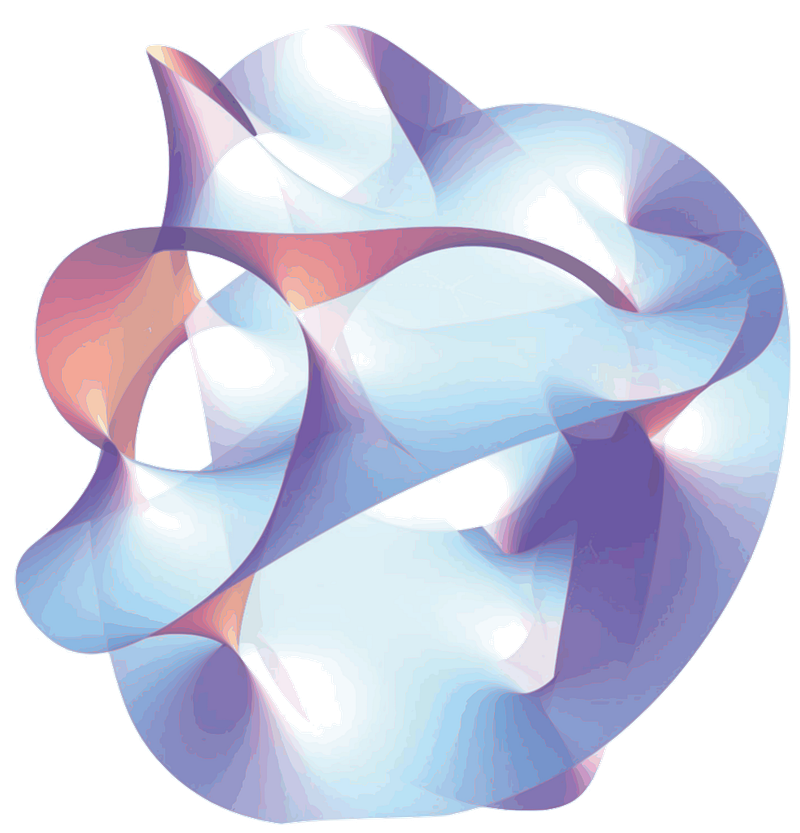
\includegraphics[width=0.35\textwidth]{reduction.png} \quad \quad}
        \vspace{2.5 cm}


        \leftline{ \small { \textbf{Internship tutors :} M. Camille Eloy}}
        \leftline{ \small { \textbf{Referent teacher :} M. Stéphane Douin}}
        \vspace{1 cm}
        \leftline{\small { \textbf{\'Educational institution :} Université Paris-Saclay / Magistère de phyisque fondamentale d'Orsay}}
        \leftline{\small { \textbf{Internship host company :}Laboratoire de Physique (UMR CNRS 5672)ENS de Lyon}}
        
        \noindent\rule[0.25\baselineskip]{\textwidth}{1pt}\\
        
        {
\includegraphics[width=0.25\textwidth]{logo.png}\quad}
        {
\includegraphics[width=0.2\textwidth]{Logo_Université_Paris-Saclay_(externe).png}\quad}\\
      
    \end{center}
\end{titlepage}
\restoregeometry


\section*{Acknowledgment}

\section*{Notations and abreviations}

We will during this intership use the vielbein formalism. We will use the same notation as in \cite{scherk1979get}
which is
\begin{itemize} \label{notation}
    \item Greek hatted letter for curved indices $(\hat \mu , \hat \nu , \hat \rho , \dots)$
    \item Latin hatted letter for flat indices $(\hat p , \hat m , \hat n , \dots)$
    \item For space-time indices taking D values, late greek letters are used in the curved case $(\mu, \nu ,\rho , \dots)$ and Latin letters in the flat case (p, m, n)
    \item For internal indices  taking E values, early Greek  letters in the curved case $(\alpha, \beta ,\gamma , \dots)$ and Latin letters in the flat case (a,b,c)
\end{itemize}
THe general coordinate $x^{ \hat\mu}$ will thereofre be made of space time coordinate $x^ \mu$ and internal coordinate $y^\alpha$. The flat lorenz
\addcontentsline{toc}{section}{Notation and abreviation }
\newpage

\tableofcontents
\clearpage
\section{Introduction}
Since the 19th-century unification of electricity and magnetism, 
and the later development of classical and quantum field theory, 
physicists have been looking for a single mathematical framework that could describe all fundamental interactions at once. 
A lot of progress has been made for the electromagnetic, 
weak and strong forces, which are now successfully unified in the Standard Model. Gravity, however, 
remains the main stumbling block. Indeed its description by General Relativity \cite{einstein1915allgemeinen} 
sits completely apart from the quantum field-theoretic language we use for everything other force.
A theory to solve this issue is to add a new symetrie to our universe, the super-symetrie. In practice this mean that we suppose a symetrie betwen fermion ,and boson. However this
symetrie come at the cost of our four dimensional universe, as it need the existense of supplementarie dimension to be possible. This new approaches is called super gravity.\\
In this internship we will begin by describing what is a field theory to seek how to describe the different action of the field we will be using, after that we will
to follow the step of \cite{scherk1979get} by doing a dimensional reduction from D+E dimension to 4 dimension. However following the step \cite{maharana1993noncompact} of we will not juste use the classical Einstein action,
but the NS-NS action of super gravity which basically add two new field. We will do this by using the vielbein formalism as it is useful for the description of fermion even here we will solely try to describe bosonics fields.
Then we will see that even if in high dimension only the SL(E,E) dimension is detectable without to much work, that when we go into law dimension another O(E,E) symetrie will apear, and 
that mean that a lot of other theory are in fact equivalent to the one we are using.\\
Finally will suppose that none of the field depend on the internal coordinate, therefor any field we will have $\partial_\alpha A^{\hat \mu} =0$

\section{Lagrangian field theory}kaluza and klein
\subsection{Lagrangian density}
In field theory, just as Newton's second law is "volumized" into the Navier-Stokes equations by distributing quantities over space, 
we replace discrete degrees of freedom with continuous field densities defined at every point in spacetime.
Therefore we will rewrite the Lagrangian as the integral over space of a new quantities called Lagrangian density, which will often refered to as just the Lagrangian.
Thus we obtain this equation:
\begin{equation} \label{densitylagrandef}
    L = \iiint \mathcal{L}(\eta_{\rho},\pdv{\eta_{\rho}}{x^{\nu}}) dx dy dz
\end{equation}
Now using esintein convention we can rewritte the action in a new light :
\begin{equation} \label{actiondensitylag}
    S = \int \mathcal{L} dx^\mu
\end{equation}

\subsection{General exemple for scalar and vectorial fields, and result for two forms}
In field theory, the Lagrangian has a classical description any field (often the simpliest).
For this work, only the scalar, vector, and two-form Lagrangians are needed, along with the metric, which is handled by Einstein's equations.\\
So for a scalar field we have : 
\begin{equation} \label{scalafield}
    \boxed{\mathcal{L} = - \frac{1}{2} \partial_\mu \Phi \partial^ \mu \Phi}
\end{equation}
and for a vectorial field we have
\begin{equation}\label{vectorialfield}
    \boxed{\mathcal{L} = - \frac{1}{}F_{\mu \nu}F^{\mu \nu}}
\end{equation}
where for the field A
\begin{equation*}
    F_{\mu \nu} = \partial_\mu A^ \nu - \partial_\nu A^ \mu
\end{equation*}
In a vaccum the einstein equation give us
\begin{equation*} \label{einsteinaction}
    \boxed{\mathcal{L} = R}
\end{equation*}
where R is ricci scalar
finally for the lagrangian of a two form fields
whe will look in \cite{maharana1993noncompact} where it is given by the equation :  
\begin{equation} \label{Baction}
    \boxed{\mathcal{L} = \frac{1}{12} g^{ \hat \mu  \mu'} g^{\nu \nu'} g^{\rho \rho'} H_{ \mu \nu \rho}H_{ \mu'\nu' \rho'}}
\end{equation}
where for the two form $B_{\nu \rho}$ we have
\begin{equation*}
    H_{ \mu \nu \rho} = \partial_ \mu B_{\nu \rho} + cyc. perm
\end{equation*}
\subsection{NS-NS Action Of supergravity}
With those object we can effectively create the NS-NS action which has this form: 
\begin{equation} \label{NS-NSaction}
    \boxed{S = \int d x^D \int \frac{d y ^E}{\rho(E)}\sqrt{- \hat g } e^{\hat \phi} (\hat R +  \hat g^{\hat \mu \hat \nu}\partial_{\hat \mu}\hat \phi \partial^{\hat \nu}\hat \phi - \frac{1}{12} g^{ \hat \mu  \mu'} g^{\nu \nu'} g^{\rho \rho'} H_{ \mu \nu \rho}H_{ \mu'\nu' \rho'})}
\end{equation} 
where $\rho(E)$ is a normalisation factor, corresponding in practice to the invariant volume of the internal space.\\
And where $\hat R$ is similar as the classical Hilbert-Einstein action but in $D+E$ dimension, $\hat \phi$ is a dilaton field and $- \frac{1}{12} H_{ \mu \nu \rho}H^{ \mu\nu \rho}$ is the  action of a two form.
Finally as no field depend on internal component and knowing what $\rho(E)$ we can just simplify this integral.
Now we will separate this action into 3 part one for each action so we have
Now that we have this action in $D+E$ dimension we need to in the same way as in the \cite{scherk1979get} reduce it, which basically mean look on how would a D dimensional observer
would perceives those extra dimension.
\subsection{different part of the action}
We can separate the action into two main componant one being the gravitional part with the dilaton and the otherone being the two forms part so we have:
\begin{subequations}
    \begin{align}
        &S_{\hat g} = \int d x^D\sqrt{- \hat g } e^{-\hat \phi} \hat  [R +\hat g^{\hat \mu \hat \nu}\partial_{\hat \mu}\hat \phi \partial^{\hat \nu}\hat \phi]\label{Sg},\\ 
        &S_{\hat B} =  \int d x^D \sqrt{- \hat g } e^{-\hat \phi} - \frac{1}{12} H_{ \mu \nu \rho}H^{ \mu\nu \rho}, \label{SB}
    \end{align}
\end{subequations}
\section{gravitional action reduction}
We will begin with the gravitional part of the NS-NS action.
\subsection{Rewriting the action}
For this part we don't need the $\hat g^{\hat \mu \hat \nu}\partial_{\hat \mu}\hat \phi \partial^{\hat \nu}\hat \phi$ part of the action so we will fully ignore it.
Now using the fact that $\hat R$ can be written as
\begin{equation*} \label{Ricciexp}
    \hat R = \hat V^{\hat \mu \hat r} \hat V^{\hat \nu \hat s} \hat R_{\hat \mu \hat \nu \hat r \hat s}
\end{equation*}
where 
\begin{equation*} \label{expriemann}
    \hat R_{\hat \mu \hat \nu \hat r \hat s} =  \partial_{\hat \mu } \hat \omega_{\hat \nu \hat r \hat s}+ \hat \omega_{\hat\mu \hat r}{}^{\hat t}\omega_{\hat\nu \hat t \hat s} - (\mu \leftrightarrow \nu)
\end{equation*}
and the $\omega$ are defined By
\begin{equation*} \label{expomega}
    \hat \omega_{trs } = - \hat\Omega_{\hat t\hat r \hat s} +\hat\Omega_{\hat r\hat s \hat t } -\hat\Omega_{\hat s\hat t \hat r}
\end{equation*}
and finally the $\Omega$ are defined thanks to the vielbein with
\begin{equation*}\label{expOmega}
    \hat\Omega_{\hat r\hat s \hat t } = \frac{1}{2}\hat (V^{\hat \mu}_{\hat r}\hat V^{\hat \nu}_{\hat s} -\hat V^{\hat \nu}_{\hat r} \hat V^{\hat \mu}_{\hat s})\partial_{\hat \nu} \hat V_{\hat \mu \hat r}
\end{equation*}
with all of that we are going to rewrite the action $S_{\hat g}$ in termes of $\hat \omega$
\begin{equation}
    \begin{aligned}
        S_{\hat g} &= \int d x^D\hat V  e^{-\hat \phi} \hat R\\
        &= \int d x^D\hat V  e^{-\hat \phi} \hat V^{\hat \mu \hat r} \hat V^{\hat \nu \hat s} \hat R_{\hat \mu \hat \nu \hat r \hat s}\\
        &= \int d x^D\hat V e^{-\hat \phi} \hat V^{\hat \mu \hat r} \hat V^{\hat \nu \hat s} ([\partial_{\hat \mu } \hat \omega_{\hat \nu \hat r \hat s} -\partial_{\hat \nu } \hat \omega_{\hat \mu \hat r \hat s}]+ [\hat \omega_{\hat\mu \hat r}{}^{\hat t}\omega_{\hat\nu \hat t \hat s} - \hat \omega_{\hat\nu \hat r}{}^{\hat t}\omega_{\hat\mu \hat t \hat s}])\\
        &= \int d x^D\{  2\hat V e^{-\hat \phi} \hat V^{\hat \mu \hat r} \hat V^{\hat \nu \hat s}\partial_{\hat \mu } \hat \omega_{\hat \nu \hat r \hat s}+ \hat V e^{-\hat \phi}[\hat \omega^{\hat r}{}_{\hat r}{}^{\hat t}\omega^{\hat s}{}_{\hat t \hat s} - \hat \omega^{\hat s}{}_{ \hat r}{}^{\hat t}\omega^{\hat r}{}_{ \hat t \hat s}] \}\\
        &= \int d x^D\{  \hat V e^{-\hat \phi}[\hat \omega^{\hat r}{}_{\hat r}{}^{\hat t}\omega^{\hat s}{}_{\hat t \hat s} - \hat \omega^{\hat s}{}_{ \hat r}{}^{\hat t}\omega^{\hat r}{}_{ \hat t \hat s}]- 2 \hat \omega_{\hat \nu \hat r \hat s}\partial_{\hat \mu}(\hat V e^{-\hat \phi} \hat V^{\hat \mu \hat r} \hat V^{\hat \nu \hat s}) \}\\
        &= \int d x^D\{  \hat V e^{-\hat \phi}[\hat \omega^{\hat r}{}_{\hat r}{}^{\hat t}\omega^{\hat s}{}_{\hat t \hat s} - \hat \omega^{\hat s}{}_{ \hat r}{}^{\hat t}\omega^{\hat r}{}_{ \hat t \hat s}]- 2\hat \omega_{\hat \nu \hat r \hat s}[\hat V e^{-\hat \phi} \hat V^{\hat \mu \hat r} \partial_{\hat \mu} \hat V^{\hat \nu \hat s} +\hat V e^{-\hat \phi}  \hat V^{\hat \nu \hat s} \partial_{\hat \mu}\hat V^{\hat \mu \hat r}+ e^{-\hat \phi} \hat V^{\hat \mu \hat r} \hat V^{\hat \nu \hat s} \partial_{\hat \mu}\hat V +\hat V  \hat V^{\hat \mu \hat r} \hat V^{\hat \nu \hat s} \partial_{\hat \mu}e^{-\hat \phi} ] \}\\
        &= \int d x^D\hat V e^{-\hat \phi} \{  \hat \omega^{\hat s}{}_{\hat s}{}^{\hat t}\omega^{\hat r}{}_{\hat r \hat t} + \hat \omega^{\hat s \hat t}{}_{ \hat r}\omega^{\hat r}{}_{  \hat s \hat t }+ 2\hat \omega_{\hat s}{}^{\hat r \hat s}\hat V^{\hat \mu}_{ \hat r}\partial_{\hat \mu}\hat \phi \}\\
    \end{aligned}
\end{equation}
\subsection{Vielbein Anstaz} \label{part:vielbeinanstaz}
Now that we have explicitely written the action in terme of either latin connexion and or the two other fields, what we hate to do is to suppose an anstaz for the vielbein. Why the vielbein and not the metric you may ask? Because as stated in  \ref{spinconnexionvielbeinandflatspace},
all the information of the metric can be contained within the vielbein, and has we primarly work with them for the action, it is easier to do an anstaz on them. Now we will do the same anzasts as in the \cite{scherk1979get},
however we will consider that $\gamma $ they use is null since the begining, and we will use the the same parameter number as in \cite{maharana1993noncompact}. Finally thank to the local lorentz invariance we can choose a triangular paremtrisation giving us
\begin{equation} \label{vielbeinanstaz}
    \boxed{\hat V^{\hat r}_{\hat \mu} =\begin{pmatrix}
    V^{r}_{\mu} & A^{(1)\beta }_{\mu} \Phi^{a}_{\beta} \\ 0 & \Phi^{a}_\alpha
    \end{pmatrix}   }
\end{equation}
Now still using \eqref{inversviel} we can compute the inverse vielbein and then the metric and then the inverse metric that gave us
\begin{equation} \label{expinverseviel}
    \hat V^{\hat r}_{\hat \mu} = \begin{pmatrix} 
         V^\mu_r &  - A^{\alpha }_r \\ 0 & \Phi^\alpha_a
    \end{pmatrix},
\end{equation}
for the inverse vielbein, and
\begin{equation} \label{expmetric}
    \hat g_{\hat \mu \hat \nu} = \begin{pmatrix}
        g_{\mu \nu} - A^{\gamma}_{\mu}A_{\nu \lambda} & - A_{\mu \beta} \\  A_{\nu \alpha} &-h_{\alpha \beta}
    \end{pmatrix}, \text{ and }
    \hat g^{\hat \mu \hat \nu} = \begin{pmatrix}
        g^{\mu \nu}  & - A^{\mu \beta} \\ - A^{\nu \alpha} &-h^{\alpha \beta}+ A^{\beta}_{\rho}A^{\rho \alpha}
    \end{pmatrix},
\end{equation}
for the metric\\
\subsection{Gauge observation} \label{part:gaugeviel}
Now that we have done the anstaz, we would like to know what each object are, for that we can use the classical gauge transformation $x'^\mu = x^\mu + \xi^\mu(x)$, and use the fact that it can be easly rewriten as a Lie derivative.
 Indeed we already know of different object transform under Lie derivative so we would easily be able indentify what each object are.\\
 So firstly let's list every known transformation:
 \begin{align} \label{xitransfo}
    &\delta \phi(x) = \xi ^ \mu \partial _ \mu \Phi (x), \\
    &\delta U ^ \mu  = \xi ^ \rho \partial _ \rho U ^ \mu - (\partial _ \rho \xi ^ \mu) U ^\rho, \\
    &\delta  \omega _ \mu  = \xi ^ \rho \partial _ \rho \omega _\mu + (\partial _ \rho \xi ^ \mu) \omega _\rho, \\
    &\delta T ^ \mu _ \nu  = \xi ^ \rho  \partial _ \rho T ^ \mu _ \nu -(\partial _ \rho \xi ^ \mu ) T ^ \rho _ \nu + (\partial _ \nu \xi ^ \rho)T ^ \mu _ \nu, 
\end{align} 
we now apply the form transformation to each block of the vielbein, in order to see whether it corresponds to some familiar type of field still thanks to \eqref{xitransfo} . Let us start with the block $\hat V^r_\mu$:
\begin{align*}
    \delta \hat V^r_\mu &= \delta V^r_\mu=  \xi^{\hat \rho}  \partial_{\hat \rho} \hat V^{ r}_{ \mu} + \partial_{ \mu} \xi^{ \hat \rho} \hat V^{  r}_{\hat \rho} \\
   &=  \xi^{\hat \rho}  \partial_{\hat \rho} \hat V^{ r}_{ \mu} + \partial_{ \mu} \xi^{ \hat \nu} \hat V^{  r}_{\hat \nu}\\
   &=  \xi^{ \rho}  \partial_{ \rho}  V^{ r}_{ \mu} + \partial_{ \mu} \xi^{  \nu}  V^{  r}_{ \nu}\\
\end{align*}
which is exactly the transformation law of a vector field under a Lie derivative \cite{freedman2012supergravity}. Applying the same method to the other blocks, we obtain, for $\Phi^a_\alpha$:
\begin{equation*}
    \delta \Phi^a_\alpha = \xi^\rho \partial_\rho \Phi^a_\alpha
\end{equation*}
which is exactly the transformation law of a scalar field. Finally, for $A^\alpha_\mu$ we obtain:
\begin{equation*}
    A^\alpha_\mu= \xi^\rho\partial_\rho A^\alpha_\mu + \partial_\mu \xi^\rho A^\alpha_\rho +\partial_\mu \xi^\alpha
\end{equation*}
which corresponds to the transformation law of a vector field, up to an extra correction term. One may further note that, restricting to $\xi^\alpha$ only, we obtain
\begin{subequations}
\begin{align}
&\delta V^r_\mu = \delta \Phi^a_\alpha = 0,\\
&\delta A^\alpha_\mu = \partial_\mu \xi^\alpha.
\end{align}
\end{subequations}
so that what remains of the $D$-dimensional diffeomorphisms, once restricted to $\xi^\alpha$ independent of the internal coordinates $y$, corresponds to a set of $E$ abelian gauge symmetries.
The vielbein in \eqref{vielbeinanstaz} thus contains the $D$-dimensional vielbein (i.e. the graviton), $E$ vector fields $A^\alpha_\mu$, and $E^2$ scalar fields $\Phi^a_\alpha$. However, because of the local Lorentz invariance in the internal directions, only $\frac{1}{2}E(E+1)$ of these scalars actually correspond to propagating degrees of freedom. We also introduce $\delta = det \Phi$ 
\subsection{Ricci scalar reduction}
Now that we better know the tool  we will use, We can begin the calculation. For a starter we will do the Einstein action in D+E dimension twiked by the addition of the dilation.\\
Firstly let's begin by expending completly the $S_{\hat g}$, this will show us that we technically have to compute 8 $\omega$, however thanks to the antisymetrie og the last to index we can reduce that to 6.
So the action is
\begin{equation} \label{Sdexp}
\boxed{
  \begin{aligned}
S=&-\frac{1}{4\kappa^{2}}\int d^{D}x\int\frac{d^{E}y}{\rho(E)}\,\hat V\,\Big[\;
\hat\omega^a{}_{b  c}\hat \omega^{bc}{}_a
-\hat \omega^a{}_{t  b}\hat \omega^{bt}{}_a
+\hat\omega^a{}_{s  c}\hat\omega^{sc}{}_a
+\hat\omega^a{}_{s  t}\hat\omega^{st}{}_a
-\hat\omega^r{}_{b  c}\hat\omega^{b}{}_r{}^c
-\hat\omega^r{}_{t  b}\hat\omega^{bt}{}_r
-\hat\omega^r{}_{s  c}\hat\omega^{s}{}_r{}^c \\
&\hat\omega^r{}_{s  t}\hat\omega^{st}{}_r
+\hat\omega^a{}_{ac}\hat\omega^b{}_b{}^c
+\hat\omega^a{}_{ta}\hat\omega^b{}^t{}_b
+\hat\omega^a{}_{ac}\hat\omega^s{}_s{}^c 
-\hat\omega^a{}_{ta}\hat\omega^s{}_s{}^t
+\hat\omega^r{}_{rc}\hat\omega^b{}_b{}^c
-\hat\omega^r{}_{rt}\hat\omega^b{}^t{}_b
+\hat\omega^r{}_{rc}\hat\omega^s{}_s{}^c
+\hat\omega^r{}_{rt}\hat\omega^s{}_s{}^t+\\
&2\hat \omega_{ s}{}^{ r  s}\hat V^{ \mu}_{  r}\partial_{ \mu}\hat \phi
+2\hat \omega_{ b}{}^{ r  b}\hat V^{ \mu}_{  r}\partial_{ \mu}\hat \phi
\;\Big]
\end{aligned}}
\end{equation}
It then becomes clear that we only need to compute six components of $\omega$, namely
\begin{align*}
    &\hat \omega_{pmn}, \;
    \hat \omega_{pma}, \;
    \hat \omega_{pab},\\
    &\hat \omega_{cmn},\;
    \hat \omega_{cma},\;
    \hat \omega_{cab},\;
\end{align*}
One can also check that computing these six components only requires the following eight components of $\Omega$:
\begin{align*}
    &\hat \Omega_{pmn},\\
    &\hat \Omega_{pma},\;
    \hat \Omega_{pam},\;
    \hat \Omega_{apm},\\
    &\hat \Omega_{mab},\;
    \hat \Omega_{amb},\;
    \hat \Omega_{abm},\\
    &\hat \Omega_{abc},
\end{align*}
Using \eqref{expinverseviel}, \eqref{expomega} and \eqref{expOmega}, we can now set out a clear strategy: first the $\Omega$'s, and then the $\omega$'s.
Now let's begin the computation of the $\Omega$'s. Starting with $\hat \Omega_{pmn}$:
\begin{align*}
    \hat \Omega_{pmn} &= \frac{1}{2}(\hat V^{\hat \mu}_{  p} \hat V^{ \nu}_{m}-\hat V^{\hat \mu}_{m} \hat V^{ \nu}_{p})\partial_{ \nu} \hat V_{\hat \mu n}\\
    &= \frac{1}{2}(\hat V^{ \mu}_{  p} \hat V^{ \nu}_{m}-\hat V^{ \mu}_{m} \hat V^{ \nu}_{p})\partial_{ \nu} \hat V_{ \mu n}\\
    &= \frac{1}{2}(\hat V^{ \mu}_{  p} \hat V^{ \nu}_{m}-\hat V^{ \mu}_{m} \hat V^{ \nu}_{p})\partial_{ \nu} \hat V_{ \mu n}\\
    &= \frac{1}{2}(V^{ \mu}_{  p} V^{ \nu}_{m}- V^{ \mu}_{m} V^{ \nu}_{p})\partial_{ \nu} ( V_{ \mu n})\\
    &= \frac{1}{2}(V^{ \mu}_{  p} V^{ \nu}_{m}- V^{ \mu}_{m} V^{ \nu}_{p})\partial_{ \nu}( V_{ \mu n})\\
    &= \frac{1}{2}(V^{ \mu}_{  p} V^{ \nu}_{m}- V^{ \mu}_{m} V^{ \nu}_{p})\partial_{ \nu}( V_{ \mu n})\\
    &= \frac{1}{2}(V^{ \mu}_{  p} V^{ \nu}_{m}- V^{ \mu}_{m} V^{ \nu}_{p})\partial_{ \nu}( V_{ \mu n})\\
    &= \frac{1}{2}(V^{ \mu}_{  p} V^{ \nu}_{m}- V^{ \mu}_{m} V^{ \nu}_{p})\partial_{ \nu}( V_{ \mu n})\\
\end{align*}
For $\hat \Omega_{pma}$, we find:
\begin{align*}
    \hat \Omega_{pma} &= \frac{1}{2}(\hat V^{\hat \mu}_{  p} \hat V^{ \nu}_{m}-\hat V^{\hat \mu}_{m} \hat V^{ \nu}_{p})\partial_{ \nu} \hat V_{\hat \mu a}\\
    &= -( V^{\mu}_{  p}  V^{ \nu}_{m}-  V^{ \mu}_{m} V^{ \nu}_{p})\partial_{ \nu} (A^{\alpha}_{\mu}\Phi_{a\alpha}) + ( A^\alpha_p V^{ \nu}_{m}- \hat A^{\alpha}_{m} V^{ \nu}_{p})\partial_{ \nu} (\Phi_{a\alpha})\\
    &= - (V^{ \mu}_{  p}  V^{ \nu}_{m}- V^{ \mu}_{m}  V^{ \nu}_{p})(\partial_{ \nu} (A^{\alpha}_{\mu})\Phi_{a\alpha}+\partial_{ \nu}(\Phi_{a\alpha})A^{\alpha}_{\mu}) + \kappa 1( A^\alpha_p V^{ \nu}_{m}- \hat A^{\alpha}_{m} V^{ \nu}_{p})\partial_{ \nu} (\Phi_{a\alpha}) \\
    &= - (V^{ \mu}_{  p}  V^{ \nu}_{m}- V^{ \mu}_{m}  V^{ \nu}_{p})(\partial_{ \nu} (A^{\alpha}_{\mu})\Phi_{a\alpha}+\partial_{ \nu}(\Phi_{a\alpha})A^{\alpha}_{\mu}) + (A^\alpha_p V^{ \nu}_{m}- \hat A^{\alpha}_{m} V^{ \nu}_{p})\partial_{ \nu} (\Phi_{a\alpha}) \\
    &= - (V^{ \mu}_{  p}  V^{ \nu}_{m}- V^{ \mu}_{m}  V^{ \nu}_{p})\partial_{ \nu} (A^{\alpha}_{\mu})\Phi_{a\alpha}\\
    &=  (F^\alpha{}_{pm}\Phi_{a\alpha}- \partial_\nu(V^{ \mu}_{  p}  V^{ \nu}_{m})A^{\alpha}_{\mu}\Phi_{a\alpha}+ \partial_\nu(V^{ \nu}_{  p}  V^{ \mu}_{m})A^{\alpha}_{\mu}\Phi_{a\alpha})\\
    &=  F^\alpha{}_{pm}\Phi_{a\alpha}
\end{align*}
For $\hat \Omega_{pam}$:
\begin{align*}
    \hat \Omega_{pam} &= \frac{1}{2}(\hat V^{\hat \mu}_{  p} \hat V^{ \nu}_{a}-\hat V^{\hat \mu}_{a} \hat V^{ \nu}_{p})\partial_{ \nu} \hat V_{\hat \mu m}\\
    &=\frac{1}{2}(\hat V^{\hat \mu}_{  p} \hat V^{ \nu}_{a}-\hat V^{\hat \mu}_{a} \hat V^{ \nu}_{p})\partial_{ \nu} \hat V_{\hat \mu m}\\
    &= 0
\end{align*}
The same result holds for $\hat \Omega_{apm}$.\\
For $\hat \Omega_{pab}$:
\begin{align*}
    \hat \Omega_{pab} &= \frac{1}{2}(\hat V^{\hat \mu}_{  p} \hat V^{ \nu}_{a}-\hat V^{\hat \mu}_{a} \hat V^{ \nu}_{p})\partial_{ \nu} \hat V_{\hat \mu b}\\
    &= \frac{-1}{2}\hat V^{\hat \mu}_{a}  V^{ \nu}_{p}\partial_{ \nu} \hat V_{\hat \mu b}\\
    &= \frac{1}{2} \Phi^{ \alpha}_{a}  V^{ \nu}_{p}\partial_{ \nu}  \Phi_{\alpha b}\\
    &= \frac{1}{2} \Phi^{ \alpha}_{a}  V^{ \nu}_{p}\partial_{ \nu}( h_{\alpha \beta} \Phi^{\beta}_{ b})\\
    &= \frac{1}{2} \Phi^{ \alpha}_{a}  \Phi^{\beta}_{ b}V^{ \nu}_{p}\partial_{ \nu} h_{\alpha \beta}  +\frac{1}{2} \Phi^{ \alpha}_{a}  V^{ \nu}_{p}h_{\alpha \beta}\partial_{ \nu}  \Phi^{\beta}_{ b}\\
    &= \frac{1}{2} \Phi^{ \alpha}_{a}  \Phi^{\beta}_{ b}V^{ \nu}_{p}\partial_{ \nu} h_{\alpha \beta}  +\frac{1}{2} \Phi_{\beta a}  V^{ \nu}_{p}\partial_{ \nu}  \Phi^{\beta}_{ b}\\
    &= \frac{1}{2} \Phi^{ \alpha}_{a}  \Phi^{\beta}_{ b}V^{ \nu}_{p}\partial_{ \nu} h_{\alpha \beta}  +\frac{1}{2}   V^{ \nu}_{p}\partial_{ \nu} (\underbrace{\Phi_{\beta a} \Phi^{\beta}_{ b}}_{\mathclap{ =\delta_{ab} \text{i.e is constant} constant}}) - \Phi^{\beta}_{ b} V^{ \nu}_{p}\partial_{ \nu} \Phi_{\beta a} \\
    &=\frac{1}{2} \Phi^{ \alpha}_{a}  \Phi^{\beta}_{ b}V^{ \nu}_{p}\partial_{ \nu} h_{\alpha \beta} - \Phi^{\beta}_{ b} V^{ \nu}_{p}\partial_{ \nu} \Phi_{\beta a} 
\end{align*}
For $\hat \Omega_{apb}$:
\begin{align*}
    \hat \Omega_{apb} &= \frac{1}{2}(\hat V^{\hat \mu}_{  a} \hat V^{ \nu}_{p}-\hat V^{\hat \mu}_{p} \hat V^{ \nu}_{a})\partial_{ \nu} \hat V_{\hat \mu b}\\
    &= \frac{1}{2}\hat V^{\hat \mu}_{  a} \hat V^{ \nu}_{p}\partial_{ \nu} \hat V_{\hat \mu b}\\
    &= \frac{1}{2}\hat V^{\alpha}_{  a} \hat V^{ \nu}_{p}\partial_{ \nu} \hat V_{\alpha b}\\
    &= \frac{-1}{2} \Phi^{\alpha}_{  a}  V^{ \nu}_{p}\partial_{ \nu} \Phi_{\alpha b}\\
\end{align*}
For $\hat \Omega_{abp}$:
\begin{align*}
    \hat \Omega_{abp} &= \frac{1}{2}(\hat V^{\hat \mu}_{  a} \hat V^{ \nu}_{b}-\hat V^{\hat \mu}_{b} \hat V^{ \nu}_{a})\partial_{ \nu} \hat V_{\hat \mu p}\\
    &= 0
\end{align*}
The same holds for $\Omega_{abc}$. Using \eqref{vielbeinanstaz}, we can then obtain the $\omega$'s:

\begin{subequations}
\begin{align}
&\hat\omega_{pmn} = \omega_{pmn},\\
&\hat \omega_{pma} = F^{\alpha}_{pm}\Phi_{\alpha a},\\
&\hat\omega_{pab} = \frac{1}{2}\Phi^\alpha_aV^\mu_p\partial_\mu\Phi_{\alpha \beta} - (a \leftrightarrow b),\\
&\hat\omega_{cmn} = - F^{\alpha}_{mn}\Phi_{\alpha c},\\
&\hat \omega_{cab}  = 0
\end{align}
\end{subequations}
We can now conclude this part by just computing the multiplication an look at what we got. This give us.
\begin{equation}
    \boxed{
    \begin{aligned}
    S = &\int d x^D \int V \delta( 
    \frac{-1}{4} g^{\rho \lambda} \partial_\lambda h_{\alpha \beta}\partial_\rho h^{\alpha \beta}
    +\frac{1}{4}F^{\mu \nu \alpha}F^{\beta}_{\mu  \nu}h_{\alpha \beta}+\\
    &+ R + \frac{1}{4} \partial_{\hat \mu} log(h) \partial^{\hat \mu} log(h) + \partial_{\hat \mu} log(h) \partial^{\hat \mu} \hat \phi )
\end{aligned}}
\end{equation}
We can observe some intersting things. Firtstly we can see that we have refound the classical Einstein action, coupled with E electromagnetism field. So what we can conclude is that gravity in D+E dimention is gravity in 4d plus E electromagnetism field.
and we find a few other field which will come in handy for the dilaton field reduction.
\subsection{Adding the dilaton field reduction}
For this part we will have to sum $S_{\hat g}$ and $S_{\hat \phi}$ that gave us
    \begin{equation*}
    \begin{aligned}
    S_{\hat g + \hat \phi} = &\int d x^D \int V \delta( 
    \frac{-1}{4} g^{\rho \lambda} \partial_\lambda h_{\alpha \beta}\partial_\rho h^{\alpha \beta}
    +\frac{1}{4}F^{\mu \nu \alpha}F^{\beta}_{\mu  \nu}h_{\alpha \beta}+\\
    &+ R + \frac{1}{4} \partial_{\hat \mu} log(h) \partial^{\hat \mu} log(h) + \partial_{\hat \mu} log(h) \partial^{\hat \mu} \hat \phi + \partial_{\hat \mu} \hat \phi \partial^{\hat \mu} \hat \phi )
\end{aligned}
\end{equation*}
We then introduce the shifted dilaton as 
\begin{equation}
    \phi = \hat \phi -\frac{1}{2} \log{h}= \hat \phi - \log{\delta}
\end{equation}
wich gave us
\begin{equation}
\boxed{
    \begin{aligned}
    S = &\int d x^D V e^{- \phi}(
    R -\frac{1}{4}F^{\mu \nu \alpha}F^{\beta}_{\mu  \nu}h_{\alpha \beta}+\\
    &- g^{\rho \lambda} \partial_\lambda h_{\alpha \beta}\partial_\rho h^{\alpha \beta}
    +\hat g^{\hat \mu  \hat \nu } \partial_{\hat \mu}\phi\partial_{\hat \nu}\phi)
\end{aligned}}
\end{equation} 
\section{Two form fiel reduction}
\subsection{The reduction}
For the two form we will reduce it apart from the two other field, this those not cause any problem as the action is in effect linear.\\
We can rewrite \eqref{Baction} as
\begin{align*}
    \mathcal{L_{\hat B}} &= \frac{-1}{12}(g^{ \hat \mu  \hat \mu'} g^{\hat \nu \hat \nu'} g^{\hat \rho  \hat \rho'} \hat H_{ \hat \mu \hat \nu \hat \rho} \hat H_{ \hat \mu' \hat \nu' \hat \rho'})\\
    &=\frac{-1}{12} (\hat \eta^{ \hat r \hat r'} \hat \eta^{\hat s \hat s'} \hat \eta^{\hat t \hat t'} \hat H_{ \hat r \hat s \hat t} \hat H_{ \hat r'  \hat s' \hat t'})\\
    &=\frac{-1}{12}(\hat H_{ \hat r \hat s\hat t}\hat H^{ \hat r \hat s \hat t})\\
    &=\frac{-1}{12}(\hat H_{  r  s t}\hat H^{  r  s  t} + \hat H_{  r  s c}\hat H^{  r  s  c} + \hat H_{  r  b t}\hat H^{  r  b  t} + \hat H_{  r  b c}\hat H^{  r  b  c} + \hat H_{  a  s t}\hat H^{  a  s  t} + \hat H_{  a  s c}\hat H^{  a  s  c} + \hat H_{  a  b s}\hat H^{  a  b  s} + \hat H_{  a  b c}\hat H^{  a  b  c})
\end{align*}
however thanks to to the fact that $\hat B_{\hat \mu \hat \nu}$ is antysymetric one can easly show that this imply that $\hat H_{ \hat \mu \hat \nu \hat \rho}$ is antysemtric for any neighbor index. so we obtaint
\begin{equation}
    \mathcal{L}_{\hat B} =\frac{-1}{12} (\hat H_{  r  s t}\hat H^{  r  s  t} + 3\hat H_{  r  s c}\hat H^{  r  s  c} + 3\hat H_{  a  s c}\hat H^{  a  s  c} + \hat H_{  a  b c}\hat H^{  a  b  c})
\end{equation}
and finnaly the action of B is writen as
\begin{equation} \label{Bactionexpa}
    \boxed{S_{\hat b } = - \int dx^D\sqrt{-g}e^{-\phi} \Big\lbrace  \frac{1}{12} H_{  \alpha  \beta \gamma} H^{  \alpha \beta \gamma  s  t} + \frac{1}{4} H_{  \mu   \alpha \beta} H^{  \mu   \alpha  \beta} + \frac{1}{4} H_{  \mu \nu \alpha } H^{  \mu  \nu  \alpha} + \frac{1}{12} H_{  \mu  \nu \rho}H^{  \mu  \nu  \rho} \Big\rbrace }
\end{equation}
Te absence if hat is due to the fact that we define low dimensional form as being:
\begin{subequations} \label{lowdimv}
    \begin{align}
        T^{\mu} &= V_r^\mu \hat V^r_{\hat \mu}\hat T^{\hat \mu} \\ \label{scalartrans}
        T^{\alpha} &= V_a^\alpha \hat V^a_{\hat \mu}\hat T^{\hat \mu}\\ \label{vectortrans}
        T_{\mu} &= V_\mu^r \hat V_r^{\hat \mu}\hat T_{\hat \mu}\\  \label{formtrans}
        T_{\alpha} &= V_\alpha^a \hat V_a^{\hat \mu}\hat T_{\hat \mu} \\  \label{tenstrans}
    \end{align}
\end{subequations}
so with that we obtaint\eqref{Bactionexpa}\\
Now we will compute each componant of non hated H in function of hated H\\
to begin slowly as we have seen above $\hat B_{\alpha \beta} = B_{\alpha \beta} $ and if we use the y independence we get $H_{\alpha \beta \gamma} = 0$\\
We continue with $H_{\mu \alpha \beta}$
\begin{equation}
    \begin{aligned}
        H_{\mu \alpha \beta} &= V^r_\mu  \hat V^{\hat \mu}_r \hat H_{\hat \mu \alpha \beta }\\
        & = \partial_\mu B_{\alpha \beta}
    \end{aligned}
\end{equation}
those two were quite easy howver the next two are going to be more troublesome, but we are going to introduce new object
Now for $H_{\mu \nu \beta}$
\begin{equation}
    \begin{aligned}
        H_{\mu \alpha \beta} &= V^r_\mu V^s_\nu \hat V^{\hat \mu}_r \hat V^{\hat \nu}_s \hat H_{\hat \mu \hat \nu \alpha}\\
        & = \hat H_{\mu \nu \alpha } -(A^{(1)\alpha}_\mu \hat H_{\alpha  \nu \rho}+A^{(1)\alpha}_\rho \hat H_{ \mu \alpha  \nu })\\
        &= \partial_\mu \hat B_{\nu \alpha} +\partial_\nu \hat B_{\alpha \mu}  -A^{(1)\beta}_\mu \partial_\nu \hat B_{\alpha \beta} -A^{(1)\beta}_\nu \partial_\mu \hat B_{\beta \alpha} \\
        &=  \partial_\mu \hat B_{\nu \alpha} +\partial_\nu \hat B_{\alpha \mu} -\partial_\nu  (A^{(1)\beta}_\mu \hat B_{\alpha \beta})+\partial_\nu A^{(1)\beta}_\mu  \hat B_{\alpha \beta}-\partial_\mu (A^{(1)\beta}_\nu \hat B_{\beta \alpha}) + \partial_\mu A^{(1)\beta}_\nu  \hat B_{\beta \alpha}\\
        &= \partial_\mu \hat B_{\nu \alpha} -\partial_\nu \hat B_{ \mu \alpha } -\partial_\nu  (A^{(1)\beta}_\mu \hat B_{\alpha \beta})+\partial_\nu A^{(1)\beta}_\mu  \hat B_{\alpha \beta}+\partial_\mu (A^{(1)\beta}_\nu \hat B_{ \alpha \beta}) - \partial_\mu A^{(1)\beta}_\nu  \hat B_{ \alpha \beta}\\
        &= \partial_\mu( \hat B_{\nu \alpha} + A^{(1)\beta}_\nu \hat B_{ \alpha \beta}) - \partial_\nu( \hat B_{ \mu \alpha } + A^{(1)\beta}_\mu \hat B_{\alpha \beta}) - \hat B_{\alpha \beta}(\partial_\mu A^{(1)\beta}_\nu-\partial_\mu A^{(1)\beta}_\nu)\\
        &= F^{(2)}_{\mu \nu \alpha } - \hat B_{ \alpha \beta }F^{(1)\beta}_{\mu \nu}
    \end{aligned}
\end{equation}
where
\begin{equation*}
    F^{(2)}_{\mu \nu \alpha} = \partial_\mu A_{\nu \alpha} -\partial_\nu A_{\mu \alpha},
\end{equation*}
and 
\begin{equation*}
    A^{(2)}_{\mu \alpha} =\hat B_{\mu \alpha} + B_{\alpha \beta} A^{(1)\beta}_\mu.
\end{equation*}
Finnaly for $H_{\mu \nu \rho}$ we are just going to use the exam same technic as before which gave us 
\begin{equation}
    \begin{aligned}
        H_{\mu \nu \rho} &=V^r_\mu V^s_\nu V^t_\rho  \hat V^{\hat \mu}_r \hat V^{\hat \nu}_s \hat V^{\hat \rho}_t \hat H_{\hat \mu \hat \nu \hat \rho}\\
        &= \hat H_{\mu \nu \rho} - A^{(1)\alpha}_{\mu} \hat H_{\alpha \nu \rho } - A^{(1)\alpha}_{\nu} \hat H_{\alpha \rho \mu } - A^{(1)\alpha}_{\rho} \hat H_{\alpha \mu \nu } +A^{(1)\alpha}_{\mu}A^{(1)\beta}_{\nu}\hat H_{\alpha \beta \rho }+A^{(1)\alpha}_{\nu}A^{(1)\beta}_{\rho}\hat H_{\alpha \beta \mu } +A^{(1)\alpha}_{\rho}A^{(1)\beta}_{\mu}\hat H_{\alpha \beta \nu }\\
        &= \partial_\mu B_{\nu \rho} -\frac{1}{2}(A^{(1)\alpha}_\mu F^{(2)}_{\nu \rho \alpha} + A^{(2)}_{\mu \alpha }F^{(1)}_{\nu \rho}) 
        +\partial_\nu B_{\rho \mu} -\frac{1}{2}(A^{(1)\alpha}_\nu F^{(2)}_{\rho \mu \alpha} + A^{(2)}_{\nu \alpha }F^{(1)}_{\rho \nu})
        +\partial_\rho B_{\mu \nu} -\frac{1}{2}(A^{(1)\alpha}_\rho F^{(2)}_{\mu \nu \alpha} + A^{(2)}_{\rho \alpha }F^{(1)}_{\mu \nu})
    \end{aligned}
\end{equation}
where
\begin{equation}
    B_{\mu \nu } = \hat B_{\mu \nu} +\frac{1}{2}A^{(1)\alpha}_\mu A^{(2)}_{\nu \alpha}-\frac{1}{2}A^{(1)\alpha}_\nu A^{(2)}_{\mu \alpha} -A^{(1)\alpha}_\mu B_{\alpha \beta }A^{(2)\beta}_{\nu }
\end{equation}
\subsection{Observation of gauge} \label{part:Bgauge}
Now as in part \ref{part:gaugeviel} we are going to observe the gauge rule to be sure that every object transorm as it should
so let's begin with $A^{(2)}$ which should transform with the lie derivative and under the new transformations of $B_{\mu \nu} \rightarrow B_{\mu \nu} + \partial_mu \Lambda_\nu$, so let's begin
with $A^{(2)}_{\mu \alpha}$
\begin{equation}
    \begin{aligned}
        \delta A^{(2)}_{\mu \alpha}&= \delta(\hat B_{\mu \alpha}+ B_{\alpha\beta}A^{(1)\beta}_\mu)\\
        &=\delta(\hat B_{\mu \alpha})+ \delta(B_{\alpha\beta}A^{(1)\beta}_\mu)\\
        &= \delta(\hat B_{\mu \alpha})+ \delta(B_{\alpha\beta})A^{(1)\beta}_\mu+ B_{\alpha\beta}\delta(A^{(1)\beta}_\mu)\\
        &= L_{\xi} \hat B_{\mu \alpha} + \partial_\mu \Lambda^{(2)}_{\alpha}+A^{(\beta)}_\mu L_{\xi} \hat B_{ \alpha \beta } +\hat B_{ \alpha \beta } \partial_\mu \Lambda^{(1)}_\alpha\\
        &= L_{\xi} \hat B_{\mu \alpha} + \partial_\mu \Lambda^{(2)}_{\alpha}+L_{\xi} (A^{(\beta)}_\mu \hat B_{ \alpha \beta })\\
        &=\partial_\mu \Lambda^{(2)}_{\alpha} +L_\xi A^{(2)}_{\mu \alpha}
    \end{aligned}
\end{equation}
so we have the right transformation for this object\\
Doing the same thing with $B_{\mu \nu}$ we come under the transformation 
\begin{equation}
    \delta B_{\mu \nu} = \frac{1}{2}(\Lambda^{(1)\alpha}F^{(2)}_{\mu \nu \alpha} + \lambda^{(2)}_{\alpha}F^{(1)\alpha}_{\mu \nu}),
\end{equation}
wich is exactly the good terme to compensate the addional term for the transformation of $H_{\mu \nu \rho}$
\section{Complete reduced action}
To recap we have the complete reduced action in the form
\begin{equation}
    S =  \int dx^D Ve^{-\phi} \mathcal{L},
\end{equation}
Where we decompose $S$ as $S =  S_1 + \S_2 + S_3 +S_4$, and we pose
\begin{equation} \label{eq:38}
    \boxed{
    \begin{aligned}
        S_1 &=\int dx^D Ve^{-\phi}(R +g^{\mu \nu}\partial_{\mu }\phi \partial_{\nu} \phi),\\
        S_2 &=\int dx^D Ve^{-\phi}(\frac{1}{4}g^{\mu \nu }(\partial_\mu h_{\alpha \beta}\partial_\nu G^{\alpha \beta} - h^{\alpha \beta } h^{\gamma \delta}\partial_\mu B_{\alpha \gamma} \partial_\nu B_{\beta \delta})),\\
        S_3 &= \int dx^DVe^{-\phi}(-\frac{1}{4}g^{\mu \rho}g^{\nu \lambda}(h_{\alpha\beta}F^{(1)\alpha}_{\mu \nu}F^{(1)\beta}_{\rho \lambda}+h^{\alpha \beta}H_{\mu \nu \alpha}H_{\rho \lambda \beta })),\\
        S_4 &=\int dx^D Ve^{-\phi}(-\frac{1}{12}H_{\mu \nu \rho} H^{\mu \nu \rho}).
    \end{aligned}}
\end{equation}
\section{Observation of new symmetry}
\subsection{O(E,E) group presentation}
Now for this part we are going to explore a very important part of physics research nowaday which is symetrie. In our context it will allow us to make equivalence between multpiple theory as whole. 
In the first place we can that we can we have an $SL(E,R)$ symetrie, which is every matrix $E\times E$ matrix with determinant of one. There other symetrie that we can see for exemple the fact that,
B only appear within a derivative mean that we can add a constant to it however we want, and as shown earlier in part \ref{part:Bgauge}, and in \ref{part:gaugeviel}, we have some gauge freedom that we can use as we please.
However, all those symetrie are manifest in high dimensional, what will interess us in the reduction is that it does not create nor destroy any symetrie and if we observe a new symetrie in the reduced form that mean that we have effectively discoverd a new symterie in the unreduced forme.
and following the \cite{maharana1993noncompact} we observe an O(E,E) symetrie
\begin{definition}
    Any matrices M is in O(E,E) if it is a square $E\times E$ matrices and if for the matrices
    \begin{equation*}
        \zeta = \begin{pmatrix}
            0 & 1 \\ 1 &0
        \end{pmatrix}
    \end{equation*}
    We can use this matrices as a metric for the groupe O(E,E) as it has d -1 eigenvalues and d 1 eigenvalues, in  a basis rotated from the one  with diagonal metric.\\ 
    the matrices M verify
    \begin{equation*}
        \boxed{M^T \zeta M = \zeta }
    \end{equation*}
\end{definition}
\subsection{Observation of the group}
We will now define a new matrices M which is 
\begin{equation}
    M = \begin{pmatrix}
        h^{-1} & -h^{-1}B \\Bh^{-1} & h-Bh^{-1}B
    \end{pmatrix}
\end{equation}
We will now try to rewrite the action in function of M to make in easier to see. $S_1$ is a lost cause as neither g or $\phi$ are contained within M, so let's being, with $S_2$, which
can be rewriten in a matrical form :
\begin{equation*}
    S_2 = \frac{1}{4}tr(\partial_{\mu}h^{-1}\partial^{\mu}h + h^{-1}\partial_\mu Bh^{-1}\partial^{\mu}B),
\end{equation*}
And now we are going to do a few manipulation
\begin{equation}
    \begin{aligned}
   S_2 &= \frac{1}{4}tr(\partial_{\mu}h^{-1}\partial^{\mu}h + h^{-1}\partial_\mu Bh^{-1}\partial^{\mu}B)\\
&=\frac{1}{8}tr\Big(2\partial_\mu h\partial^\mu h^{-1}+2h^{-1}\partial_\mu B h^{-1}\partial^\mu B\Big)\\
&=\frac{1}{8}tr\Big(2\partial_\mu h\partial^\mu h^{-1}-2\partial_\mu(Bh^{-1}B)\partial^\mu h^{-1}+\partial_\mu(Bh^{-1})\partial^\mu(Bh^{-1})+\partial_\mu(h^{-1}B)\partial^\mu(h^{-1}B)\Big)\\
&=\frac{1}{8}tr\Big(\partial_\mu(h-Bh^{-1}B)\partial^\mu h^{-1}+\partial_\mu(Bh^{-1})\partial^\mu(Bh^{-1})+\partial_\mu(h^{-1}B)\partial^\mu(h^{-1}B)+\partial^\mu h^{-1}\partial_\mu(h-Bh^{-1}B)\Big)\\
& = \frac{1}{8}tr(\partial_\mu M^{-1}\partial^\mu M)
    \end{aligned}
\end{equation}

Now we are going to rewrite $S_3$ by developing the H partial to get
\begin{equation}
    \begin{aligned}
    S_3 &= -\frac{1}{4}[F^{(1)\alpha}_{\mu \nu }h_{\alpha \beta}F^{(1)\mu \nu \beta}+ (F^{(2)}_{\mu\nu \alpha}-B_{\alpha \gamma}F^{(1)\gamma}_{\mu \nu})h^{\alpha \beta}(F^{(2)\mu \nu}_{\beta}-B_{\beta \delta}F^{(1)\mu \nu \delta})]\\
    &=-\frac{1}{4} \mathcal{F}^i_{\mu \nu}(M^{-1})_{ij} \mathcal{F}^{\mu \nu j}
    \end{aligned}
\end{equation}
Where $\mathcal{F}^i_{\mu \nu}$ is the 2E-component vector of field strengths
\begin{equation}
    \mathcal{F}^i_{\mu \nu} = \begin{pmatrix} F^{(1)\alpha}_{\mu \nu} \\F^{(2)}_{\mu \nu \alpha} \end{pmatrix} = \partial_\mu \mathcal{A}^i_\nu - \partial_\nu \mathcal{A}^i_\mu
\end{equation}
And finnaly we go to $S_4$ firstly let's rewrite $H_{\mu \nu \rho}$
\begin{equation}
    \begin{aligned}
    H_{\mu \nu \rho} &=\partial_\mu B_{\nu \rho} -\frac{1}{2}(A^{(1)\alpha}_\mu F^{(2)}_{\nu \rho \alpha} + A^{(2)}_{\mu \alpha }F^{(1)}_{\nu \rho}) 
        +\partial_\nu B_{\rho \mu} -\frac{1}{2}(A^{(1)\alpha}_\nu F^{(2)}_{\rho \mu \alpha} + A^{(2)}_{\nu \alpha }F^{(1)}_{\rho \nu})
        +\partial_\rho B_{\mu \nu} -\frac{1}{2}(A^{(1)\alpha}_\rho F^{(2)}_{\mu \nu \alpha} + A^{(2)}_{\rho \alpha }F^{(1)}_{\mu \nu})\\
        &= \partial_\mu B_{\nu \rho} -\frac{1}{2} \mathcal{A}^i_\mu \zeta_{ij} \mathcal{F}^j_{\nu \rho} + (cyc. perms)
      \end{aligned}
\end{equation}
We can now rewrite the complete action in terms of M, that gave us:
\begin{equation}
    \begin{aligned}
    S = &\int dx^D Ve^{-\phi}[R +g^{\mu \nu}\partial_{\mu }\phi \partial_{\nu} \phi + \frac{1}{8}tr(\partial_\mu M^{-1}\partial^\mu M)
    -\frac{1}{4} \mathcal{F}^i_{\mu \nu}(M^{-1})_{ij} \mathcal{F}^{\mu \nu j}  \\
    &- \frac{1}{12}(\partial_\mu B_{\nu \rho} -\frac{1}{2} \mathcal{A}^i_\mu \zeta_{ij} \mathcal{F}^j_{\nu \rho} + (cyc. perms))(\partial^\mu B^{\nu \rho} -\frac{1}{2} \mathcal{A}^{i\mu} \zeta_{ij} \mathcal{F}^{j\nu \rho} + (cyc. perms))]
    \end{aligned}
\end{equation}
We will know studie the effect of the $0(E,E)$ group on this action, firstly as it only act on the internal index, so the action of the group on the different part of the 
are
\begin{align}
    &g_{\mu \nu} \rightarrow g_{\mu \nu},\\
    &\phi \rightarrow \phi
\end{align}
It is worth noting that for $\phi$ the whole thing is invariant however each componant ($\hat \phi$, and $\frac{1}{2}log(h)$) on there one are not invariant to $O(E,E)$ group, which is why 
we needed to creatz the shifted dilaton.\\
We also need to define the action of the groupe on the two form, and for $A^{(2)}$, when they have internal index, so we have:
\begin{align}
    &A^i \rightarrow \Omega^i_j A^j \\
    &M_{ij} \rightarrow \Omega^l_i M_{lk}\Omega^k_j
\end{align}
Here $\Omega \in O(E,E)$. Finnaly we can show that $M \in O(E,E)$ Indeed
\begin{equation*}
    \begin{aligned}
        M^{T}\zeta M &= \begin{pmatrix} h^{-1} & B h^{-1} \\ - h^{-1} B & h-Bh^{-1}B\end{pmatrix} \begin{pmatrix}0 & 1 \\ 1 & 0\end{pmatrix}\begin{pmatrix}    h^{-1} & -h^{-1}B \\Bh^{-1} & h-Bh^{-1}B\end{pmatrix}\\
        & =\begin{pmatrix}B h^{-1}   &h^{-1}  \\h-Bh^{-1}B   &- h^{-1} B \end{pmatrix} \begin{pmatrix}    h^{-1} & -h^{-1}B \\Bh^{-1} & h-Bh^{-1}B\end{pmatrix}\\
        &= \begin{pmatrix}0 & 1 \\ 1 & 0\end{pmatrix} = \zeta
    \end{aligned}
\end{equation*}
Which mean that under 

Now as $\Omega^T \zeta \Omega = \zeta$ the seconds thermes is O(E,E) invariant. And the for the first terme is invariant if we require that $B_{\nu \rho}$ does not transfrom.
This demonstrates that the action hides a non-trivial symmetry, providing a useful framework for comparing equivalent theories.
 \section{Conclusion}
 
 \printbibliography
 \appendix
 \section{lagrangian}
 By using the principle of least action and the variational principle we can see that
\begin{align*}
    \delta S &= \delta \int \mathcal{L} dx^\mu \\
    & = \delta \int \pdv{\mathcal{L}}{\eta_{\rho}} \delta \eta_{\rho} + \pdv{\mathcal{L}}{\partial_{\nu}\eta_{\rho}} \delta \partial_ \nu \eta_{\rho}  dx^\mu\\
    & = \delta \int \pdv{\mathcal{L}}{\eta_{\rho}} \delta \eta_{\rho}- \partial_ \nu \pdv{\mathcal{L}}{\partial_{\nu}\eta_{\rho}} \delta  \eta_{\rho}  + \underbrace{\partial_ \nu \Big(\pdv{\mathcal{L}}{\partial_{\nu}\eta_{\rho}} \delta  \eta_{\rho}\Big)}_{\mathclap{\text{border terme equal to zero}}}  dx^\mu\\
    & = 0
\end{align*}
which gave the equation
\begin{equation}
    \boxed{\pdv{\mathcal{L}}{\eta_{\rho}} - \partial_ \nu \pdv{\mathcal{L}}{\partial_{\nu}\eta_{\rho}} = 0}
\end{equation}
which is in fact the equation of mouvement for the field\section{General relativty 101}
\begin{definition}
Let V be an R-vector space of dimension N, we define the tensor of order $(r,s) \in  \llbracket 0 ,1 \rrbracket^2$ on $V^{(r,s)} \overset{def}{=} V^{\otimes r} \otimes V^{\otimes s}$
as a being a multilinear application on $ V^{\star r} \times V^{ s}$ to $\mathbb{R}$
 \end{definition}
\begin{definition}
    We will call n-dimension ($n \in \mathbb{N}^*$) manifold every Hausdorff topological space $(\mathcal{M},\tau )$ localy homeomorphic to $\mathbb{R}^n)$
\end{definition}
\begin{definition}
    Let $(\mathcal{M}, g)$ be a smooth manifold. A metric tensor is a symmetric, 
    non-degenerate bilinear form $g_{\mu\nu}$ on the tangent space $T_p\mathcal{M}$ 
    at each point $p \in \mathcal{M}$, such that
    \begin{equation*}
        ds^2 = g_{\mu\nu} dx^\mu dx^\nu
    \end{equation*}
    In General Relativity we use the signature $(-,+,+,+)$.
\end{definition}
\begin{definition}
   In general in RG we use the christofells connexion as it is the sole one wich is mtreci and torsion free.\\
   We define it as being
   \begin{equation}
    \\nabla_{\mu}V^{\nu}= \partial_{\mu}V^{\nu}+\Gamma^{\nu}_{\mu \sigma}V^{\sigma}
   \end{equation} 
   where the christofells symbols are
   \begin{equation}
    \Gamma_{\mu \nu}^{\lambda} = \frac{1}{2}g^{\lambda \sigma}(\partial_{\mu}g_{\nu \sigma}+\partial_{\nu}g_{\sigma \mu} - \partial_{\sigma}g_{\mu \nu})
   \end{equation}
\end{definition}

\end{document}